%settings

\setlength{\parindent}{2ex}
\phantomsection
%text
%-Task1----------------------------------
\section{Model of the application using Deployment Diagrams}
\par
\begin{figure}[h!]
	\centering
	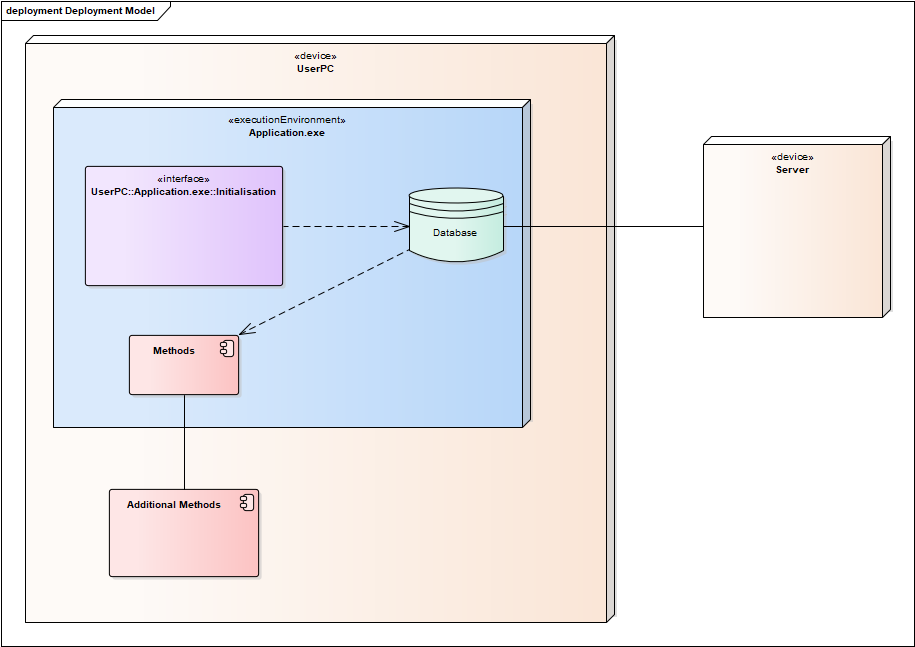
\includegraphics[width=\textwidth]{DeploymentModel}
	\caption{Class Diagram} 
\end{figure}
The application is run on the device it was installed ,it communicates with the server through database if it was connected to LAN ,the database also communicates with the Methods and tells them when to start their process.
%-Task2----------------------------------
\newpage
\section{Document the application delivery / installation.}
The application is delivered through and online shop.\par
The user is provided with a install package executable, the installer will unpack the executable, the package with the methods and a file containing the database(that will register the commands of user through the interface and the track methods tracked data).\par 
The installer will ask the user the installation directory ,ask if he wants to place a shortcut of the executable on the desktop and upon the ending of the installation will be asked if he wants to run the program.

\clearpage
